% Figure from MATH 493 notes, section 71. Compile with the notes preamble.
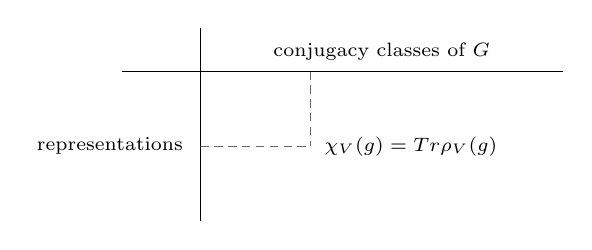
\begin{tikzpicture}[font=\scriptsize]
\draw (0,0) -- (5.6,0);
\draw (1.0,0.55) -- (1.0,-1.9);
\node[anchor=south] at (3.3,0.02) {conjugacy classes of $G$};
\node[anchor=east] at (0.9,-0.95) {representations};
\draw[densely dashed, black!60] (2.4,0) -- (2.4,-0.95);
\draw[densely dashed, black!60] (1.0,-0.95) -- (2.4,-0.95);
\node[anchor=west] at (2.45,-0.95) {$\chi_V(g) = \operatorname{Tr}\rho_V(g)$};
\end{tikzpicture}
